  
%%%%%%%%%%%%%%%%%%%%%%% file typeinst.tex %%%%%%%%%%%%%%%%%%%%%%%%%
%
% This is the LaTeX source for the instructions to authors using
% the LaTeX document class 'llncs.cls' for contributions to
% the Lecture Notes in Computer Sciences series.
% http://www.springer.com/lncs       Springer Heidelberg 2006/05/04
%
% It may be used as a template for your own input - copy it
% to a new file with a new name and use it as the basis
% for your article.
%
% NB: the document class 'llncs' has its own and detailed documentation, see
% ftp://ftp.springer.de/data/pubftp/pub/tex/latex/llncs/latex2e/llncsdoc.pdf
%
%%%%%%%%%%%%%%%%%%%%%%%%%%%%%%%%%%%%%%%%%%%%%%%%%%%%%%%%%%%%%%%%%%%


\documentclass[runningheads,a4paper]{llncs}

\usepackage{amssymb}
\setcounter{tocdepth}{3}
\usepackage{graphicx}
\usepackage{amsthm}
\usepackage{mathtools}
\usepackage{url}
\newcommand{\keywords}[1]{\par\addvspace\baselineskip
\noindent\keywordname\enspace\ignorespaces#1}
\usepackage{pifont}
\usepackage[utf8]{inputenc}
\inputencoding{utf8}

\begin{document}

\mainmatter  % start of an individual contribution

% first the title is needed
\title{Deadlocks as Runtime Exceptions}

% a short form should be given in case it is too long for the running head
\titlerunning{Deadlocks as Runtime Exceptions}

% the name(s) of the author(s) follow(s) next
%
% NB: Chinese authors should write their first names(s) in front of
% their surnames. This ensures that the names appear correctly in
% the running heads and the author index.
%
\author{Rafael Brandao Lobo%
\and Fernando Castor}

\authorrunning{Deadlocks as Runtime Exceptions}

\institute{Center of Informatics, Federal\\
University of Pernambuco, Brazil\\
{rbl,castor}@cin.ufpe.br\\
\url{http://www.springer.com/lncs}}

\toctitle{Lecturas Notes in Computer Science}
\tocauthor{Authors' Instructions}
\maketitle

\begin{abstract}
\dots
\keywords{\dots}
\end{abstract}
\chapter{Introduction}

Real-world applications use concurrency to parallelize computation in multiple threads or processes, taking more advantage of multicore processors.
However concurrenct code is difficult to write correctly, as it is well documented in \cite{lu}. In a concurrent code, for example, a developer must
take in consideration all possible interleaves that multiple threads in the running code can take which is simply not feasible.
When multiple threads access concurrently a certain memory position, data races may occur.
One way to solve this problem is to first identify parts of the code that should not allow threads to run simultaneously -- they are
called critical sections -- and then protect them by using locks. 

Locks are used to avoid data races in concurrent code. When a thread acquires a certain lock, no other thread can acquire the same lock.
Any thread that attempt to acquire that lock will be blocked until that resource is released. Once that thread finishes to execute critical code,
it should release that lock so other threads would be unblocked afterwards.

Unfortunately locks cannot be easily composed in the code and a very common bug caused by composing locks in unexpected ways is called deadlock.
A deadlock manifests when threads are waiting each other in a cycle, each one holding locks that other thread is trying to acquire.

Suppose a thread X acquires a lock A and then tries to acquire a lock B. Given the nature of parallelism, another thread Y simultaneously acquires
a lock B and then tries to acquire lock A. Since thread X is blocked waiting for lock B to be released and thread Y which owns lock B is blocked
waiting for thread X to release lock A, both will never finish waiting, thus creating a deadlock. When a deadlock happens, a program fail
to make progress without notice to users and developers, making harder to identify the problem.

Deadlocks can be avoided if locks are acquired in any order, as long as the other threads follows that particular order. For example, if both thread X
and thread Y always acquired locks A and B in this order, then no deadlock could ever occur because there's no waiting relationship cycle between them. 
Some existing techniques to avoid deadlock require to impose a global order on locks and check whether this order is ever violated when the locks are acquired \cite{marino},
but this approach is not practical for real world software because most of the time the code that acquires the first lock is unaware of wh.

There are two main types of deadlocks: resource deadlocks and communication deadlocks \cite{singhal} \cite{knapp}. Resource deadlocks are illustrated in the previous
example, where threads wait for resources to become available. Communication deadlocks happens when threads are blocked waiting messages, so messages are the resources
for which threads wait. In this work, as other studies did before \cite{mcsdk} \cite{magicfuzzer}, our focus will be on resource deadlocks and from now on and whenever the term \emph{deadlock} is used by itself we will be referring to resource deadlocks unless mentioned otherwise.

Over the time, many studies tried to solve deadlock by detecting them in many different ways which can be made by either static analysis, dynamic analysis, or a mix of them. Static analysis leverage deadlock existence by reading the source code and estimating whether a deadlock would be possible with that code without actually running it. In counter part, dynamic analysis dynamically add extra code in the original source and possibly detect real deadlocks during execution. But each one of those techniques
have its own advantages and disadvantages and they complement one another.

In this study, however, we are focusing on solving deadlocks differently. We believe deadlocks should not fail silently but instead they should be handled as exceptions in programming languages. Rather than trying to detect them when explicitly requested for a deadlock analysis, programs should instead be written in such a way that they can either handle the deadlock when it happens by deploying some custom deadlock recovery logic or just show the error in the output in order to ease finding bugs and solving them later.

There are some programming languages such as Haskell and Go that already contain some kind of deadlock exception for very particular cases. In this study, the proposed deadlock exception was focused on what we've found out to be the most common type of deadlock: the classical deadlock illustrated in the previous example where only two threads are involved and they're waiting circularly for two resources.

\section{Summary of Goals}

In this work we have the main goal to show how deadlock detection between two threads and two locks can be implemented with very low runtime overhead and evaluate the impact of deadlock exceptions on the efficiency of identifying deadlocks in software by running an empirical study with students. With this contribution, we seek to understand the benefits of such exceptions in programming languages and also offer a lightweight implementation of deadlock exceptions that can seamlessly run on top of Java OpenJDK.

\section{Outline}

The remainder of this work will be organized as follows:

\begin{itemize}
  \item Chapter 2 discuss the basic concepts of deadlock exceptions, highlighting previous studies and terms that are necessary to understand before proceeding to the next chapters.
  \item Chapter 3 presents our study on bug reports in open source projects, focusing on deadlock bugs and identifying some of its characteristics.
  \item Chapter 4 shows our deadlock detection algorithm in details, presenting a sketch of a formal proof, what changes were done to Java's ReentrantLock and a quick performance evaluation.
  \item Chapter 5 discuss the empiric evaluation we did to measure efficiency of deadlock exceptions on identifying bugs in software.
  \item Chapter 6 presents the contributions of this work, discusses some related and future work, and presents our main conclusions.
  \item Appendix A shows the code used to calculate the size of sample we've used in Chapter 3.
  \item Appendix B shows the code used to analyse the data collected in Chapter 3.
  \item Appendix C shows the code used to collect the data from different repositories used in Chapter 3.
  \item Appendix D shows Java's ReentrantLock pseudocode cited in Chapter 4.
  \item Appendix E shows R instructions to evaluate time used in Chapter 5.
  \item Appendix F shows input for R script used to analyse time in Chapter 5.
\end{itemize}




\section{Deadlock Detection}

In this section we present the proposed approach. We extend the notion of lock by making locks responsible for both detecting TTTL deadlocks and raising exceptions whenever such deadlocks occur. In this section we present an algorithm implementing this extended notion of lock and show that our algorithm guarantees that (i) every TTTL deadlock is detected; and (ii) if an exception reporting a deadlock is raised, it must stem from the occurrence of a TTTL deadlock.

We have modified the default implementation of Java's \emph{ReentrantLock} to allow efficient runtime detection of TTTL deadlocks. It works as follows:

\begin{enumerate}
\item Each lock has a pointer to a thread, the owner of the lock, or {\tt null} when no thread owns that lock.
\item Each lock has an integer to represent its current state: 0 means the lock is free and no thread owns it (the \emph{unlocked} state), 1 means there is a thread that owns the lock (the \emph{locked} state). For simplicity, we are only interested on these two states. Nonetheless, in the implementation of \emph{ReentrantLock}, each time a thread owner acquires the same lock, this state would be incremented, and decremented each time the thread releases it.
\item Each thread has a thread-local list of pointers to locks it currently owns.
\item Each lock has a waiting queue of threads that are waiting to acquire it. Whenever a thread tries to obtain a lock when it's already acquired, the thread will add itself to the waiting queue before parking. Upon the event of releasing the lock, the owner of that lock will look for the first thread in the waiting queue and unpark it.
\item When a thread wants to acquire a lock, it will swap the current state to \emph{locked} if the current state is \emph{unlocked} atomically.
\begin{enumerate}
\item If the thread fails, it must be because the lock is already owned by some other thread, then it will add itself on the waiting queue for that lock. Finally, the thread will park.
\item Otherwise, the thread will set itself as the current owner of that lock and also add this lock to its thread-local list of pointers of locks it owns.
\end{enumerate}
\item When a thread is about to release a lock, the current owner pointer of that lock is set to {\tt null} and that lock is also removed from the thread-local list of owned locks. Finally, the lock state is changed to \emph{unlocked}.
\item Before parking, a thread will check whether there is a deadlock. When the current thread is unable to acquire its desired lock, it must be because another thread already owns it. It is possible to know who is the owner of any lock, so the current thread identifies the owner of its desired lock as the conflicting thread. Then the current thread will search on each lock of its list of owned locks if the conflicting thread is waiting for it.
\begin{enumerate}
\item If positive, then we have a circular dependency (current thread is stuck waiting for its desired lock and the conflicting thread is stuck waiting for a lock the current thread owns) and thus a deadlock exception will be raised.
\item Otherwise, the thread parks.
\end{enumerate}
\end{enumerate}

We take advantage of the current algorithm employed by \emph{ReentrantLock} and some of its guarantees listed below to avoid the need to introduce extra synchronization mechanisms or costly atomic operations during deadlock detection:
\begin{enumerate}
\item The operation of swapping the state of a lock from \emph{unlocked} to \emph{locked} must be done atomically by the thread, so only one thread can be successful at a time.
\item A thread will only park when it is guaranteed that some other thread can unpark it. Missing notifications will never happen and concurrent uses of park and unpark on the same thread will be resolved gracefully.
\item Inserts on each lock's waiting queue must be done atomically. If multiple threads concurrently attempt to insert themselves in the waiting queue on the same lock, they will both succeed eventually but the exact order of insertions is not important.
\item Once the last element in the waiting queue of a lock is read, it should be safe to read all threads in the waiting queue that arrived before the last element. Since the thread who reads the waiting queues is also the one who blocks every thread waiting on the queues, we can guarantee the only updates that could happen concurrently are new insertions at the end of each queue. However insertions in the end of the queue are not important once a last element pointer is obtained.
\end{enumerate}

%Now we show why this algorithm works:%

\begin{lemma}
The proposed protocol can always detect TTTL deadlocks.
\end{lemma}
\begin{proof}
By way of contradiction, suppose not and a TTTL deadlock occurred without it being detected.
Lets assume that threads \emph{A} and \emph{B} have both acquired locks \emph{a} and \emph{b} respectively, as follows:
\begin{equation}
write_{A}(state_{a} = locked) \rightarrow write_{A}(owner_{a} = A)
\end{equation}
\begin{equation}
write_{B}(state_{b} = locked) \rightarrow write_{B}(owner_{b} = B)
\end{equation}
In the above expressions, `$x \rightarrow y$' indicates that event $x$ happened before event $y$. Notation `$write_{B}(owner_{b} = B)$' indicates that thread $B$ wrote to variable $owner_{b}$ the value $B$. 
And now each thread will attempt to acquire the opposing lock: thread \emph{A} is trying to acquire lock \emph{b} and thread \emph{B} is trying to acquire lock \emph{a}, as follows:
\begin{equation}
read_{A}(state_{b} == locked) \rightarrow write_{A}(waiting\_queue_{b}.insert(A))
\end{equation}
\begin{equation}
read_{B}(state_{a} == locked) \rightarrow write_{B}(waiting\_queue_{a}.insert(B))
\end{equation}
The notation `$read_{A}(state_{b} == locked)$' indicates that thread $A$ read variable $state_{b}$ and obtained value $locked$.
If a TTTL deadlock happened, then both threads are now parked and all previous equations should be correct.
But before parking, each thread must check for deadlock by inspecting each lock it owns if the opposing thread is on its waiting queue.
As we initially assumed no deadlock exception has been raised, then both threads are parked and also the following equations must be correct:
\begin{equation}
read_{A}(owner_{b} == B) \rightarrow read_{A}(waiting\_queue_{a}.contains(B) == false)
\end{equation}
\begin{equation}
read_{B}(owner_{a} == A) \rightarrow read_{B}(waiting\_queue_{b}.contains(A) == false)
\end{equation}
The problem with the previous equations is that they both cannot be true simultaneously.
Before checking for deadlock, each thread must add itself on the waiting queue of its desired lock.
If it holds that the opposing thread is not in the waiting queue yet, then it must be because it did not start to check for deadlock yet, thus a contradiction.
\end{proof}

\begin{lemma}
The proposed protocol never raises a deadlock exception for a non-existent TTTL deadlock.
\end{lemma}
\begin{proof}
By way of contradiction, assume the opposite: a deadlock exception was raised and there is no real TTTL deadlock. Exactly one of the following equations must be true in order to raise a deadlock exception (if both were true at the same time, an actual deadlock would have occurred):
\begin{equation}
read_{A}(owner_{b} == B) \rightarrow read_{A}(waiting\_queue_{a}.contains(B) == true)
\end{equation}
\begin{equation}
read_{B}(owner_{a} == A) \rightarrow read_{B}(waiting\_queue_{b}.contains(A) == true)
\end{equation}
Suppose without loss of generality that the first equation is true.
It means that thread \emph{B} is waiting for lock \emph{a} and it is also the owner of lock \emph{b}.
If it is on the waiting queue, that thread is either parked already or about to park
and in both cases thread \emph{B} is going to depend on the release of lock \emph{a} to proceed.
However, as we have seem previously, thread \emph{A} at this point is also about to park and is checking for a deadlock.
If this condition holds, we have a circular dependency between threads \emph{A} and \emph{B}, a real TTTL deadlock, thus we have a contradiction.
\end{proof}

\subsection{Extension: raising exceptions in all threads}

The protocol we presented guarantees that an exception is raised in at least one of the threads involved in a deadlock. A safer approach, however, would be to have exceptions raised in both threads involved in the deadlock. In this section we describe an extension to the protocol that provides this guarantee. This does not affect how deadlock is detected but what should be done after a deadlock is detected. Thus, does not impact the correctness of the protocol. The proposed extension comprises the following:

\begin{enumerate}
\item Each lock has a list of tainted threads. This list should only be read or updated by the owner of that lock, allowing immunity from interference without any extra synchronization cost.
\item Once a deadlock is detected and the current thread is about to raise a deadlock exception, it already knows which thread is conflicting with itself and which lock that thread desires. The current thread (the owner of the desired lock) will add this conflicting thread to the tainted threads list for that lock. After that, the deadlock exception is raised.
\item When the conflicting thread is unparked and finally acquires its desired lock (it becomes the owner of that lock), then it is allowed to read the list of tainted threads. If this thread identifies itself in this list, then it must be because it was part of a deadlock before, so it removes its reference from the list and also raises a deadlock exception.
\item Every operation on the list of tainted threads of any lock (either reading or inserting values) should be followed up by some cleanup on all references to threads that are no longer running.
\end{enumerate}

That is sufficient to force both threads to raise exceptions when only one of them would raise an exception in the initial protocol. The latter only raises exception on both threads if they simultaneously reach the point where they check for deadlocks. However, for this particular case, this change introduces a different problem: dangling references.
If each thread adds their conflicting thread to the lists of tainted threads of the locks they own, 
but none of them is able to acquire their respective desired locks (as in \emph{item 3}),
both threads will leave their references behind for others to cleanup (as in \emph{item 4}).
We minimize this issue by cleaning these references as soon as any thread acquires the lock.

\subsection{Implementation}

The full version of the modified OpenJDK \emph{ReentrantLock} that implements this algorithm is available in our code repository~\cite{repo}.
In this section we will focus on what changes were done, so we will present pseudo-code to illustrate.

\medskip
\noindent
{\it Changes on ReentrantLock: keep ownedLocks list updated}
\begin{verbatim}
// This is a thread-local inside a lock.
// Each thread keeps the list of locks they own.
DEFINE_PER_THREAD(List<Lock>, ownedLocks);

// As soon as a lock is acquired or release, this function is called.
// Based on that, we call register or unregister owned lock.
void setExclusiveOwner(Thread thread) {
  owner = thread;
  if (owner == null) {
    unregisterOwnedLock();
  } else {
    registerOwnedLock();
  }
}

// These functions register or unregister the current lock
// in the thread-local list ownedLocks.
registerOwnedLock();
unregisterOwnedLock();
\end{verbatim}

Following the first part of the protocol, we must keep a list of locks each thread owns.
This list is thread-local so it's free from interference (each thread will only manage its own list).
Method calls to \emph{setExclusiveOwner} are intercepted to also update the list of owned locks accordingly as follows:
whenever the call resets the owner it means there was a release, so we unregister that lock and removes it from the list of owned locks of the current thread;
futhermore, we do the opposite when the owner is not null, as it means that the thread has owned that lock and it should update its own list of owned locks to add that particular entry.

\medskip
\noindent
{\it Changes on ReentrantLock: detect deadlock and throw exception}
\begin{verbatim}
void park() {
  Thread conflictingThread = owner;
  if (isAnyOwnedLockDesiredBy(conflictingThread)) {
    clearOwnedLocksByCurrentThread();
    throw new DeadlockException();
  }
  LockSupport.park(this);
}

// Returns true if any of the locks owned by the current thread
// contain a given thread in the waiting queue.
isAnyOwnedLockDesiredBy(Thread);

// Clear all locks in the list of owned locks by the current thread.
clearOwnedLocksByCurrentThread();
\end{verbatim}

When a thread attempts to acquire a lock and this lock is already owned, we deploy the deadlock check right before the thread actually get parked.
It starts by checking which thread is the owner of this particular lock, then the current thread checks whether there's any lock owned by itself
that is currently being waited by that conflicting thread. If positive, then we have a circular wait so we must throw a deadlock exception.
Next step is to guarantee that both threads will receive the deadlock exception.

\medskip
\noindent
{\it Changes on ReentrantLock: throw deadlock exception on both threads}
\begin{verbatim}
// Each lock will have a list of threads that are not allowed to
// acquire this lock (if it happens, throw exception).
DEFINE_PER_LOCK(List<Thread>, taintedThreads);

void park() {
  Thread conflictingThread = owner;
  List<Lock> desiredLocks =
    getOwnedLocksDesiredBy(conflictingThread);
  if (!desiredLocks.isEmpty()) {
    foreach(Lock k in desiredLocks) {
      k.taintedThreads.add(conflictingThread);
    }
    clearOwnedLocksByCurrentThread();
    throw new DeadlockException();
  }
  LockSupport.park(this);
}

// Returns a list of locks owned by the current thread where
// a particular Thread (passed as parameter) is waiting for.
getOwnedLocksDesiredBy(Thread);

// Add a check as soon as a thread acquires this lock.
// If it is marked as tainted, then throw exception.
void setExclusiveOwner(Thread thread) {
  owner = thread;
  if (owner == null) {
    unregisterOwnedLock();
  } else {
    registerOwnedLock();
    if (taintedThreads.contains(thread)) {
      clearOwnedLocksByCurrentThread();
      throw new DeadlockException();
    }
  }
}

\end{verbatim}

We expand the algorithm by adding a list of threads on each lock object that will contain threads that just went into a deadlock and should also throw exception as soon as possible.
When a deadlock is detected, the following case was possible: one thread throws an exception and releases all its locks, then the second thread would finally acquire its desired lock
which should be free after the first thread released its locks.

The solution to force the second thread to also throw an exception was to observe that the at the point where the first thread is about to throw an exception, the second thread
is already stuck waiting for the first thread. Also, the first thread is still the owner of the current lock object allowing it to modify the list of tainted threads inside that lock.
Then it updates tainted threads list by adding the second thread on it. Next time the second thread acquires this lock, it will throw an exception too.

There's a small disadvantage of this final solution which is a leak of Thread references on taintedThreads objects for each lock. It can happen when both threads
simultaneously detect the deadlock and both throw exceptions. In this case, they would have added the opposite thread inside their own lock's taintedThreads list, but afterwards
both threads would stop and none of them would attempt to acquire the opposite lock again. We've minimized the effect of this leak by also removing non-active thread
references from taintedThreads list every time any update is done on this list, so in practice other threads would eventually clean up them. The code which minimizes this
leak is available on our repository \cite{repo}, but for the sake of brevity we've not included it here.

\subsection{Performance Overhead}\label{sec:perf}

We conducted a preliminary set of experiments to analyze the overhead of our approach.
We compared the our implementation of ReentrantLock with deadlock exceptions, the original ReentrantLock and Eclipse's {\tt OrderedLock}~\cite{orderedlock} implementation in a synthetic benchmark.

OrderedLock is a deadlock-safe implementation of a lock which relies on Eclipse's code architecture.
It is similar our approach in the sense that it attempts to detect deadlocks at runtime. However, it aims to be general, detecting $N$-thread deadlocks without much concern for performance: when a deadlock happens, it releases all locks by a given thread and suspends it, allowing other threads to proceed;
later, the suspended thread will acquire such locks again.
Since it allows threads to temporarily give up all its owned locks, it loses the property of guaranteeing exclusive access policy in \emph{critical zones} that all locks should provide.
In order to use it in our evaluation, as it deeply relies on Eclipse's code architecture to function, we had to perform some small code changes, removing only Eclipse-specific bits that did not affect the core functionality of OrderedLock.
The source code for these lock implementations is available elsewhere~\cite{repo}.

We developed a synthetic benchmark that creates \emph{N} threads that perform additions to ten integer counters where each increment in a counter is protected by explicit locks. Each thread would have to increment its corresponding counter 1000 times before finishing its execution and the counters were evenly distributed across the threads. Therefore, each counter will have exactly \emph{(N / 10)} threads doing increments on it and higher values of \emph{N} result in higher contention, that is, more threads will compete against each other for a particular counter. In this preliminary evaluation, we have conducted measurements for values of $N$ equal to 10, 50, 100, and 200. Since each thread in the benchmark never acquires more than one lock at the same time, deadlocks cannot occur. We emphasize that this setup is very conservative, since every operation that each thread performs requires locking. Thus, the obtained overhead will be a worst-case estimate and thus much higher than one would encounter in a real-world application~\cite{lozi}. The measurements were made on an Intel CoreTM i7 3632QM Processor (6Mb Cache, 2.2GHz) running Ubuntu 12.04.4 LTS and each cell in Table~\ref{tab:overhead} is the average of 50 executions (preceded by 20 executions that served as a warm-up).

\begin{table}
\begin{center}
\caption{Benchmark time measurements (in seconds)}\label{tab:overhead}
\begin{tabular}{|l|l|l|l|}
\hline
\# Threads & ReentrantLock & ReentrantLock Modified & OrderedLock \\
\hline
10 & 0.084184 & 0.105729 & 0.159503\\
50 & 0.089094 & 0.136507 & 1.094718\\
100 & 0.090978 & 0.159541 & 3.395974\\
200 & 0.131739 & 0.194075 & 11.258714\\
\hline
\end{tabular}
\end{center}
\end{table}

The difference of results between our implementation and the original ReentrantLock gives a range of increased time from about 50\% to 90\%. Meanwhile, OrderedLock performed a lot worse, reaching a 8446.3\% increase in time for the worst case. To get a rough estimate of the impact that this overhead would have on actual application execution time, we analyzed the results obtained by Lozi et al.~\cite{lozi}. The authors profiled 19 real-world applications and small benchmarks in order to measure the time these systems spend on their critical sections. Worst-case results ranged between 0.3\% and 92.7\%. If we consider the average time spent on the critical sections of 12 of these systems, the impact of our approach on the overall execution time would be \textbf{less than 6\% in the worst case}. The remaining cases are extreme, in the sense that these systems spend more time in their critical sections than out of them~\cite{lozi}. 


\section{Evaluation}

In this chapter we present an evaluation of our approach. Our evaluation comprises two parts: (i) a usability evaluation involving two experiments with two groups of students (Section~\ref{sec:usab}); and (ii) a preliminary analysis of the performance overhead of our approach (Section~\ref{sec:perf}).  The exact input, instructions, and any additional document we have used in this section are available in appendices or in our repository~\cite{repo}.

\subsection{Usability Evaluation}\label{sec:usab}

We ran empirical evaluation to measure the efficiency of deadlock exceptions with regard to problem solving speed and accuracy. We defined two research questions for this evaluation: 

\begin{itemize}
\item {\bf RQ1.} Is the time spent to identify the bug reduced using our implementation?
\item {\bf RQ2.} Is the accuracy in the identification of the causes of a deadlock bug improved for developers using our approach?
\end{itemize}

The metric we watched to answer the first question was the time (in seconds) to finish each question in the test. For the second question, the metric we used was the number of correct answers. We evaluated students answers under different criteria (see Table~\ref{tab:crit}), where each one received a score that was either 0, 0.5 or 1, where 0 means the criteria was not met at all, 0.5 means it was partially met, and 1 means it was complete. Whenever $(A - B) + C \geq 1.5$ was true, we defined it as a correct answer; that is, whenever the bug was described as deadlock and at least one of the methods involved in the deadlock were identified correctly. We didn't use criteria \emph{D} and \emph{E} because in our questions statements, we didn't make it clear that we wanted description of all locks involved in the deadlock; also, our deadlock implementation at that time only guaranteed at least one thread raising deadlock exception thus affecting at least one method. In other words, this equation means that an answer was correct whenever the bug was described as deadlock, did not contain any affirmation saying it was another type of bug, and at least one of the methods involved were identified.

\begin{table}
\begin{center}
\caption{Criteria to evaluate students answers}\label{tab:crit}
\begin{tabular}{|l|l|}
\hline
Criteria & Description \\
\hline
A & Correctly classified problem as deadlock \\
B & Classified problem as different from deadlock  \\
C & Correctly identified method calls involved in the deadlock \\
D & Correctly identified locks involved in the deadlock  \\
E & Pointed unrelated methods as part of the deadlock \\
\hline
\end{tabular}
\end{center}
\end{table}

\subsubsection{Time Analysis.}

We defined the following hypothesis to answer {\bf RQ1}:

\begin{equation}
  H_{0} : \mu_{TimeLockA} \geq \mu_{TimeLockB}
\end{equation}
\begin{equation}
  H_{1} : \mu_{TimeLockA} < \mu_{TimeLockB}
\end{equation}

\subsubsection{Design, Instrumentation and Subjects.}

In order to prevent \emph{bias}, we needed to control a few factors during the experiment execution. The first factor was the selection of subjects to participate on this experiment, as different background knowledge could potentially influence chosen metrics. The second factor we had to control was the complexity of programs that each subject would have to look into. Complexity was interpreted as a direct relation to the amount of files in the program, number of threads and number of locks to analyze; as we've assumed that easier programs could have little or no benefit from deadlock exceptions, we wanted to have one program that we considered easy to identify the problem and another that was more complex and composed by many files and classes, reflecting a more realistic case. We provided implementations of each program using either \emph{LockA} or \emph{LockB}: the two possible treatments that we wanted to compare.

We decided to use Latin Square Design~\cite{box} to control these two factors mentioned earlier: subjects and program complexity factors. Since we had N subjects, 2 programs and 2 possible treatments, we disposed subjects in rows and programs in columns of latin squares, randomly assigning in each cell of the square a treatment that could be \emph{LockA} or \emph{LockB}, but also guaranteeing that for any given row or column in this square, each treatment appears only once (see Table~\ref{tab:latin}). Consequently, we have replication, local control and randomization which are the three principles of experiment design \cite{box}.

\begin{table}
\begin{center}
\caption{Latin Square design}\label{tab:latin}
\begin{tabular}{|l|l|l|}
\hline
 & Program 1 & Program 2\\
\hline
Subject 1 & LockA & LockB\\
Subject 2 & LockB & LockA\\
\hline
\end{tabular}
\end{center}
\end{table}

We wrote two programs with different complexity which were presented in the same order for all subjects. The first program, known as \emph{Bank}, contained 4 classes spread in 4 files, 3 threads, 3 explicit locks, and 82 lines of code in average. The second program, known as \emph{Eclipse} had 15 classes spread in 11 files, 4 threads, 5 explicit locks, and 40 lines of code in average. We expected the first program to be easier to identify the deadlock because it contained fewer classes and files. Each program could use either \emph{LockA} or \emph{LockB} but we randomly assigned a group to each student so that if they fall into group A, they would start with \emph{LockA} in the first question, but change to \emph{LockB} on the second question; or if they fall in group B, they they would start with \emph{LockB} and switch to \emph{LockA} in the second question. We randomly paired subjects in tuples composed of one subject in group A and another subject of group B, then we created latin squares for each one of these pairs, where any remainders were discarded.

% TODO: insert each program description here, where the deadlock was, etc. in the end, point to where the source for each pdf is %

We repeated this experiment twice.
The two experiments had similar setups but differed in terms of the subjects. For the first experiment, the subjects comprised a group of third-year undergraduate students who underwent an 18-hour concurrent programming course. The course included a number of programming assignments. The experiment was conducted as a test for the course. The subjects of the second experiment were  graduate students enrolled in master's degree or PhD program attending a 40-hour Parallel Programming course with a focus on algorithms and data structures. They had classes about advanced concepts of parallel programming and had practical exercises, including implementing a number of different locking approaches. The participants in the second experiment were all volunteers and were not required to take part in it. Also, for both experiments, the assignments were the same. It asked students to identify any problems they could with the provided programs.

%We did a survey with the second group to understand their background even further (see charts below) at the end of the experiment. TODO: insert chart with survey results

\subsubsection{Metrics Collection.}

All students started the experiment with program \emph{Bank}. When they finished, they received the second program, \emph{Eclipse}. When a student finished one of the programs, we set a timestamp on it, or in a few cases, we allowed students to do it by themselves but we had to double check the values and fix in case there was any error. The timestamp was written based on a chronometer visible to everyone in the laboratory. For the first group (undergraduate students), we allowed 90 minutes per program. For the second group (graduate students), we allowed 60 minutes per program. 

Each one should start the experiment with the first question containing \emph{Program 1} and once they finish to provide an answer, they should request for the second question. At that point, we collect and place a timestamp in their answer. Once they finish the second question containing \emph{Program 2}, then they should again give us a notice so we can leave a new timestamp. Later we used these timestamps to measure how long they took to finish each question. We have started this experiment with a time limit for each question of 60 minutes each. However, during the first experiment, students complained and we realized it would not be sufficient for all students so we expanded to 90 minutes.

The timestamp was written by students conducting the experiment based on a counter we projected on the laboratory wall in real time. In a few circunstances the subject could write the timestamp when they finished, but we have double checked the value at the time we collected their answer, overwriting in case they did any mistake.

\subsubsection{Experiment Operation.}

We executed this experiment in two different days. In the first day we did it with undergraduate students in replacement of their default exam, so their participation was obligatory but we disclaimed they could optionally leave a comment if they did not want to take part in this research, so we would not use their data. Fortunately no one chose to not participate. In the second day, we did it with graduate students after the last class of Parallel Programming course and it was optional. In total, 31 students participated on the first day and 16 students participated on the second day, but we had to discard 2 students data because they arrived late and they had to leave early.

On the first day we started with a time frame of 2 hours for the whole experiment, so we decided to set a deadline for each question and put a time limit of 1 hour each. Later we expanded the time limit to 1 hour 30 minutes for each question. On the second day we decided to stick with 1 hour each because there was no demand to extend it.

\subsubsection{Results.}

Time analysis was conducted with R Statistical Software using the inputs extracted from each day.
We used the linear model described in Figure~\ref{fig:model} that considers the effect of different factors
on the response variable as proposed by other authors~\cite{paola}~\cite{sanchez}.

\begin{figure}
\begin{center}
$Y_{lijk} = \mu + \tau_{l} + \tau\alpha_{li} + \beta_{j} + \gamma_{k} + \tau\gamma_{lk} + \epsilon_{lijk}$\\
\vspace{4mm}
\begin{tabular}{ll}
$Y_{lijk}$ & - response of $l_{th}$ replica, $i_{th}$ student, $j_{th}$ program, $k_{th}$ lock \\
$\tau_{l}$ & - effect of $l_{th}$ replica \\
$\tau\alpha_{li}$ & - effect of interaction between $l_{th}$ replica and $i_{th}$ student \\
$\beta_{j}$ & - effect of $j_{th}$ program \\
$\gamma_{k}$ & - effect of $k_{th}$ lock \\
$\tau\gamma_{lk}$ & - effect of interaction between $l_{th}$ replica and $k_{th}$ lock \\
$\epsilon_{lijk}$ & - random error \\
\end{tabular}
\caption{Regression model.}\label{fig:model}
\end{center}
\end{figure}

Initially, we've plotted box-plot graphic (Figure~\ref{fig:boxplot1}) and calculated the average time spent to solve tasks for both groups (Table~\ref{tab:mean1}).
They show that students using {\tt LockB} took more time to complete the tasks.
On Figure~\ref{fig:boxplot1}, we can see time spent for both groups stop at nearly the same point, and we believe the reason behind it is that we enforced a time limit for each question.
If there was no such time limit on each question, we believe that {\tt LockB} time spent range would be significantly wider.

\begin{figure}
\centering
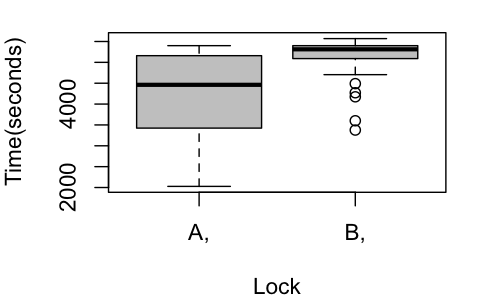
\includegraphics[height=4.5cm]{img/u1.png}
\caption{First experiment box-plot graphic.}\label{fig:boxplot1}
\end{figure}

\begin{table}
\centering
\begin{tabular}{|l|l|l|}
\hline
 & Time Spent (seconds)\\
\hline
LockA & 4227.800 \\
LockB & 5086.367 \\
\hline
\end{tabular}
\caption{First experiment's average time spent}\label{tab:mean1}
\end{table}

Then we run the Box-Cox transformation - a power transformation - to reduce anomalies such as non-additivity and non-normality.
First we verify if the transformation is needed, obtaining the curve in the left of Figure~\ref{fig:transf1}.
Since the value of {\tt lambda} at the maximum point in the curve is not approximately 1, we should apply it.
In order to apply the transformation, $Y_{lijk}$ should be powered to that $\lambda$ on our regression model.
Now, using the transformed model, we obtain the curve shown in the right of Figure~\ref{fig:transf1}.

\begin{figure}
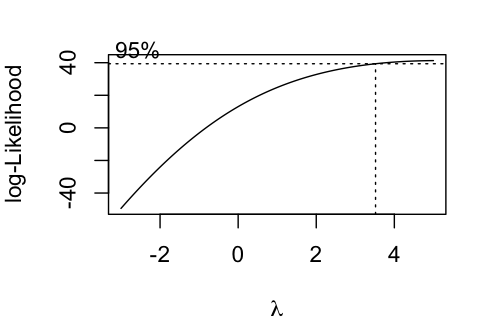
\includegraphics[height=4.5cm, width=6cm]{img/u2.png}
\hfill
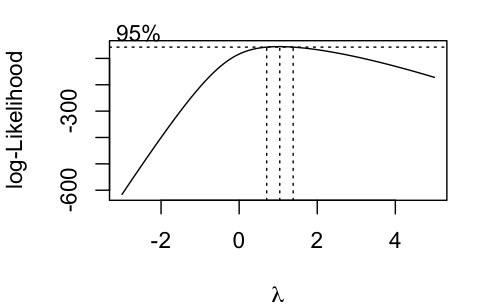
\includegraphics[height=4.3cm, width=6cm]{img/u2boxcox.png}
\caption{First experiment: before and after box-cox transformation ($\lambda = 5$).}\label{fig:transf1}
\end{figure}

In the next step we ran Tukey Test of Additivity to check whether effect model was additive.
Interaction between factors displayed on rows and columns of each latin square won't affect significantly the response only when the model is additive~\cite{box},
so we must verify it (Figure~\ref{tab:tukey}).

\begin{figure}
\centering
\begin{tabular}{ll}
$H_{0}$ & : The model is additive \\
$H_{1}$ & : $H_{0}$ is $false$ \\
\end{tabular}
\caption{Tukey Test of Additivity hypothesis}\label{tab:tukey}
\end{figure}

When the test was executed, we obtained p-value of 0.514, which means we cannot reject $H_{0}$.
Consequently the model was considered to be additive.

Finally, we ran the ANOVA (ANalysis Of VAriance) test which compares the effect of treatments on the response variable,
providing an approximated p-value for every associated factor (see Table~\ref{tab:anova1}).
When a variable has p-value $< 0.05$, it means that factor was statistically significant to the response.
It shows that {\bf lock factor was the most significant to the response}, allowing us to reject our null hypothesis defined in Equation 10.

\begin{table}
\begin{center}
\caption{Undergraduate students experiment ANOVA results.}\label{tab:anova1}
\begin{tabular}{|l|l|l|l|l|ll|}
\hline
                & Df &    Sum Sq  &  Mean Sq   & F value & \emph{p-value} &     \\  
Replica         & 14 & 3.8633e+37 & 2.7595e+36 & 1.6553  & 0.1784197 &     \\   
Program         & 1  & 4.1460e+36 & 4.1460e+36 & 2.4869  & 0.1371197 &     \\   
Lock            & 1  & 3.9489e+37 & 3.9489e+37 & 23.6873 & 0.0002492 & *** \\
Replica:Student & 15 & 4.1013e+37 & 2.7342e+36 & 1.6401  & 0.1808595 &     \\  
Replica:Lock    & 14 & 2.4033e+37 & 1.7166e+36 & 1.0297  & 0.4785520 &     \\  
Residuals       & 14 & 2.3340e+37 & 1.6671e+36 &         &           &     \\
\hline
\end{tabular}
\end{center}
\end{table}

Now we will show the results collected by the second experiment with graduate students. They were exposed to the same set of problems in a different day, but as explained before, they only had a time limit of 1 hour per question.

When we analyze the box-plot for the second group (Image~\ref{fig:boxplot2}) and their average time spent (Table~\ref{tab:mean2}), we can see there was a clear improvement on the time for students using \emph{LockA}.

\begin{figure}
\centering
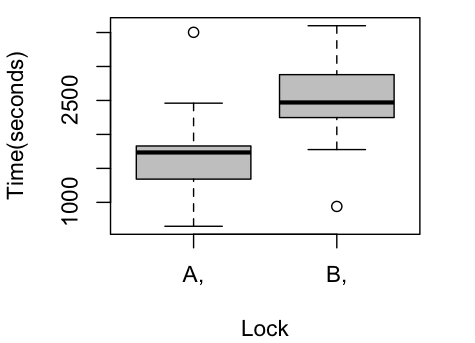
\includegraphics[height=4.5cm]{img/g1.png}
\caption{Second experiment box-plot graphic.}\label{fig:boxplot2}
\end{figure}

\begin{table}
\centering
\begin{tabular}{|l|l|l|}
\hline
 & Time Spent (seconds)\\
\hline
LockA & 1737.714 \\
LockB & 2507.714 \\
\hline
\end{tabular}
\caption{Second experiment's average time spent}\label{tab:mean2}
\end{table}

Moving foward with the analysis, we check if a box-cox transformation is needed. Since the value is not approximately 1, we apply the power transformation the same way we did with the first experiment, but with the corresponding lambda value.

\begin{figure}
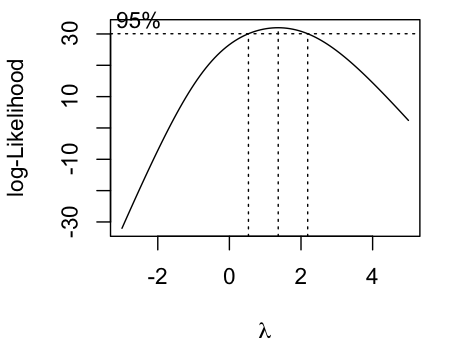
\includegraphics[height=4.5cm]{img/g2.png}
\hfill
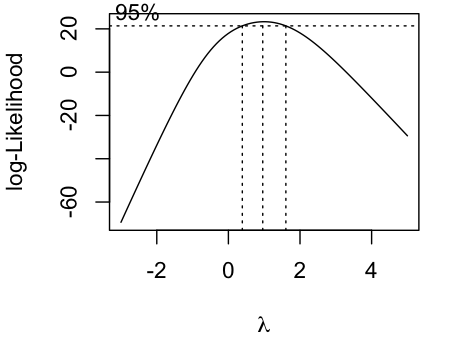
\includegraphics[height=4.4cm]{img/g2boxcox.png}
\caption{Before and after box-cox transformation ($\lambda = 1.3636$).}\label{fig:transf2}
\end{figure}

Finally, running ANOVA, we can see that the type of lock was the most significant factor for the response time, as shown in Table~\ref{tab:anova2}. Again, we can reject the null hypothesis.

\begin{table}
\begin{center}
\caption{Graduate students ANOVA results.}\label{tab:anova2}
\begin{tabular}{|l|l|l|l|l|ll|}
\hline
                 & Df &    Sum Sq &   Mean Sq  & F value &   Pr(>F) & \\   
\hline
replica          & 6 & 2576883250 &  429480542 & 14.1891 & 0.0025793 & **  \\
program          & 1 &    6875586 &    6875586 &  0.2272 & 0.6505035 &     \\
lock             & 1 & 1958179433 & 1958179433 & 64.6938 & 0.0001975 & *** \\
replica:student  & 7 & 2328154077 &  332593440 & 10.9881 & 0.0047601 & **  \\
replica:lock     & 6 &  823830276 &  137305046 &  4.5362 & 0.0441188 & *   \\
Residuals        & 6 &  181610625 &   30268438 &         &           &     \\
\hline
\end{tabular}
\end{center}
\end{table}

\subsubsection{Accuracy Analysis.}

We used the number of correct answers using each lock to measure accuracy, so we defined the following hypothesis to answer {\bf RQ2}. 

\begin{equation}
  H_{0} : \mu_{CorrectAnswersLockA} \leq \mu_{CorrectAnswersLockB}
\end{equation}
\begin{equation}
  H_{1} : \mu_{CorrectAnswersLockA} > \mu_{CorrectAnswersLockB}
\end{equation}

Once we collected all answers, we manually evaluated each one of them according to the criterias established previously, where each criteria had an associated value between 0 and 1. Then we've ran a script that evaluates the equation we defined before to classify whether an answer was correct or not. Grouping the results in tables, we have Table~\ref{tab:acc1} and Table~\ref{tab:acc2}.

\begin{table}
\begin{center}
\caption{Undergraduate students answers accuracy}\label{tab:acc1}
\begin{tabular}{|l|l|l|}
\hline
 & Correct & Incorrect\\
\hline
LockA & 29 & 2\\
LockB & 16 & 15\\
\hline
\end{tabular}
\end{center}
\end{table}

\begin{table}
\begin{center}
\caption{Graduate students answers accuracy}\label{tab:acc2}
\begin{tabular}{|l|l|l|}
\hline
 & Correct & Incorrect\\
\hline
LockA & 13 & 1\\
LockB & 10 & 4\\
\hline
\end{tabular}
\end{center}
\end{table}

Applying Fisher's exact test we can see that undergraduate students results presented a two-tailed P value equals 0.0004: the association between rows (groups) and columns (outcomes) is considered to be extremely statistically significant; consequently, there is clear evidence of improvement on accuracy (see Table~\ref{tab:acc1}).

Meanwhile graduate students results presented a two-tailed P value equals 0.3259, which does not represent a statistically significant evidence of improvement in accuracy (see Table~\ref{tab:acc2}).

% TODO: add script and the data used (anonymized) to appendices or put on github and link %

\subsection{Discussion}

% TODO: review this section, it was written based on older results %

We can see in our results that both groups of students have improved their time to solve the problem when they had the lock with deadlock exception. Also, on the first group, we have found statistically significant evidence that it improved answers accuracy, but not for the second group.

We cannot draw conclusions regarding the improved accuracy on the second group, but we can bring up some relevant aspects we've observed and make a few hypothesis. Some students in the second group were greatly experienced on concurrent programming and they knew how to efficiently find a deadlock using the tools available in Eclipse. Thus, they have finished the exercise really quickly for both problems, knowing exactly which points in the code were involved in the deadlock. So we can see that deadlock exceptions are more helpful for unexperienced programmers in general, and it's possible that even if we had a bigger sample for the second group, we would still not see a significant difference that would indicate deadlock exceptions improved their accuracy.

However, we believe that the benefits of deadlock exceptions are beyond helping unexperienced programmers to find deadlocks more precisely. Experienced programmers would still benefit in many cases where the deadlock is not as obvious as in the exercise we've presented. For example, in a more realistic situation, a deadlock can happen in a background thread that doesn't really affect the program execution overall but make the execution lacking some expected behavior. Furthermore, in non-interactive systems where they are only running in background, is nearly impossible to know when there's a problem unless this software is monitored constantly which is very time consuming or the system produces output constantly that is affected by a potential deadlock. If we have a deadlock exception, we can either prepare and handle this exception on the code level, or just have this signal from output that would help developers to fix it later.

\subsection{Threats To Internal Validity}

In this experiment, we've collected evidence on how the presence of deadlock exception affects student ability to identify deadlocks accurately. However, we must raise a few considerations regarding the validity of our results.

\subsubsection{Time Measurement.}

Since we wanted to run the experiment in a homogenous environment, we've decided to run it in a laboratory in Federal University of Pernambuco, and we've provided links to download the exercise and a few instructions explaining how to deploy it. We wanted to make it as easy as possible and before we've started the test, we gave a small presentation reproducing step by step the instructions that would be described on each exercise, so everyone could follow up and make the setup at the same time. Once everyone was done, we've started to count the time and allowed them to run the programs and start debugging. However, this procedure was not enough: there was a few students (approximately 3 in total) who did the setup differently and could not execute the program; therefore, they've lost a few minutes until we've fixed that for them. Since they've lost only a few minutes, we have still counted them as part of the experiment and did not discount the time.

Furthermore, some students arrived at the test more than 10 minutes late. We've allowed them to join, but some of the remaining computers in the laboratory had issues like they were not logging in or the mouse was not working. We've lost a few minutes to make them work or find a new computer and once each of them did the setup, we've started to count their time individually.

Whenever a student finished a given question, if the time was below the time limit they had available, we have marked the current timestamp on each student's name in the whiteboard. Each entry inserted was already sorted by time, so we easily tracked whether each student was close to the second question's time limit. It would have been better to do this automatically rather than doing manually, so we could potentially reduce overhead of these timestamp operations and increase their precision.

Also, we believe that our imposed time limit have limited more drastically the time ranges on the first group because they spent more time on each question. Also the fact it was an exam for them may have delayed the time to answer because they were more careful. We have observed during the experiment that many students wrote their answers but they were reluctant to ask for the next question because they still have plenty of time left and they wanted to make sure it was correct. We did not observe such behavior with the second group of students and we believe it is because they did not have the same pressure to deliver correct results as the first group had.

\subsubsection{Exercises.}

We understand that the two questions we've used to evaluate the students are far easier than what most software engineers have to deal with in the real world. However we could not use any real world issue because it would easily take the time limit of the experiement for each bug.

On the other hand, we've created two questions based on real world bugs that we have found while searching for deadlock bugs in open source repositories. Each question had a particular level of granularity, where one should be easier to find a bug because of the less amount of code to examine and another that should be more difficult because of the reasonable amount of different files to look at.

Some researchers actually believe that empiric evaluations should not be limited to real projects. Buse claims there are benefits of using non-real artifacts \cite{buse} because it's easier for researchers to translate research questions into successful experiments as it allows a greater control over confouding factors. Otherwise, it would be necessary to turn all participants familiar with the codebase of a real and complex system before even starting the experiment. 

\subsection{Threats to External Validity}

Let's consider a few conditions that might limit the generalization power of our findings in this experiment.

\subsubsection{Students.}

Each student which participated in this experiment had a different background. What we did to minimize the differences was to select groups where students had at least basic experience in concurrent programming and they should be familiarized with the types of bugs such codes can have: the first group of students with undergraduate students attended the class Paradigms of Computaional Languages where deadlocks are covered in classes and exercises; the second group with graduate students attended the class Parallel Programming which covered concurrent programming in low level detail in classes and exercises, including deadlock detection.

Some studies have already addressed the problem of drawing conclusions made with students but some suggest that using students as subjects is as good as using industry professionals \cite{staron}. Runes ran an experiment which shows that there's not much significant differences between undergraduate, graduate and industry professionals, with the exception that undergraduate students often take more time to complete the tasks \cite{runes}.

\subsection{Performance Overhead}\label{sec:perf}

We conducted a preliminary set of experiments to analyze the overhead of our approach.
We compared the our implementation of ReentrantLock with deadlock exceptions, the original ReentrantLock and Eclipse's {\tt OrderedLock}~\cite{orderedlock} implementation in a synthetic benchmark.

OrderedLock is a deadlock-safe implementation of a lock which relies on Eclipse's code architecture.
It is similar our approach in the sense that it attempts to detect deadlocks at runtime. However, it aims to be general, detecting $N$-thread deadlocks without much concern for performance: when a deadlock happens, it releases all locks by a given thread and suspends it, allowing other threads to proceed;
later, the suspended thread will acquire such locks again.
Since it allows threads to temporarily give up all its owned locks, it loses the property of guaranteeing exclusive access policy in \emph{critical zones} that all locks should provide.
In order to use it in our evaluation, as it deeply relies on Eclipse's code architecture to function, we had to perform some small code changes, removing only Eclipse-specific bits that did not affect the core functionality of OrderedLock.
The source code for these lock implementations is available elsewhere~\cite{repo}.

We developed a synthetic benchmark that creates \emph{N} threads that perform additions to ten integer counters where each increment in a counter is protected by explicit locks. Each thread would have to increment its corresponding counter 1000 times before finishing its execution and the counters were evenly distributed across the threads. Therefore, each counter will have exactly \emph{(N / 10)} threads doing increments on it and higher values of \emph{N} result in higher contention, that is, more threads will compete against each other for a particular counter. In this preliminary evaluation, we have conducted measurements for values of $N$ equal to 10, 50, 100, and 200. Since each thread in the benchmark never acquires more than one lock at the same time, deadlocks cannot occur. We emphasize that this setup is very conservative, since every operation that each thread performs requires locking. Thus, the obtained overhead will be a worst-case estimate and thus much higher than one would encounter in a real-world application~\cite{lozi}. The measurements were made on an Intel CoreTM i7 3632QM Processor (6Mb Cache, 2.2GHz) running Ubuntu 12.04.4 LTS and each cell in Table~\ref{tab:overhead} is the average of 50 executions (preceded by 20 executions that served as a warm-up).

\begin{table}
\begin{center}
\caption{Benchmark time measurements (in seconds)}\label{tab:overhead}
\begin{tabular}{|l|l|l|l|}
\hline
\# Threads & ReentrantLock & ReentrantLock Modified & OrderedLock \\
\hline
10 & 0.084184 & 0.105729 & 0.159503\\
50 & 0.089094 & 0.136507 & 1.094718\\
100 & 0.090978 & 0.159541 & 3.395974\\
200 & 0.131739 & 0.194075 & 11.258714\\
\hline
\end{tabular}
\end{center}
\end{table}

The difference of results between our implementation and the original ReentrantLock gives a range of increased time from about 50\% to 90\%. Meanwhile, OrderedLock performed a lot worse, reaching a 8446.3\% increase in time for the worst case. To get a rough estimate of the impact that this overhead would have on actual application execution time, we analyzed the results obtained by Lozi et al.~\cite{lozi}. The authors profiled 19 real-world applications and small benchmarks in order to measure the time these systems spend on their critical sections. Worst-case results ranged between 0.3\% and 92.7\%. If we consider the average time spent on the critical sections of 12 of these systems, the impact of our approach on the overall execution time would be \textbf{less than 6\% in the worst case}. The remaining cases are extreme, in the sense that these systems spend more time in their critical sections than out of them~\cite{lozi}. 




\chapter{Bibliography}

\begin{thebibliography}{4}

\bibitem{lu} Lu, Shan, et al: Learning from mistakes: a comprehensive study on real world concurrency bug characteristics.
ACM Sigplan Notices. Vol. 43. No. 3. ACM, 2008.

\bibitem{singhal} Singhal, Mukesh. Deadlock detection in distributed systems.
Computer 22.11 (1989): 37-48.

\bibitem{knapp} Knapp, Edgar: Deadlock detection in distributed databases.
ACM Computing Surveys (CSUR) 19.4 (1987): 303-328.

\bibitem{marino} Marino, Daniel, et al: Detecting deadlock in programs with data-centric synchronization.
Software Engineering (ICSE), 2013 35th International Conference on. IEEE, 2013.

\bibitem{dolby} Dolby, Julian, et al: A data-centric approach to synchronization.
ACM Transactions on Programming Languages and Systems (TOPLAS) 34.1 (2012): 4.

\bibitem{mcsdk} Da Luo, Zhi, Raja Das, and Yao Qi: Multicore sdk: a practical and efficient deadlock detector for real-world applications.
Software Testing, Verification and Validation (ICST), 2011 IEEE Fourth International Conference on. IEEE, 2011.

\bibitem{tanter} Tanter, Éric, et al: Altering Java semantics via bytecode manipulation.
Generative Programming and Component Engineering. Springer Berlin Heidelberg, 2002.

\bibitem{contest} ConcurrentTesting - Advanced Testing for Multi-Threaded Java Applications, \url{https://www.research.ibm.com/haifa/projects/verification/contest/}

\bibitem{magicfuzzer} Cai, Yan, and W. K. Chan: MagicFuzzer: scalable deadlock detection for large-scale applications.
Proceedings of the 2012 International Conference on Software Engineering. IEEE Press, 2012.

\bibitem{pin} Luk, Chi-Keung, et al. Pin: building customized program analysis tools with dynamic instrumentation.
ACM Sigplan Notices 40.6 (2005): 190-200.

\bibitem{mysql} MySQL, available at: \url{http://www.mysql.com}

\bibitem{firefox} Firefox, available at \url{http://www.mozilla.org/firefox}

\bibitem{chromium} Chromium, available at \url{http://code.google.com/chromium}

\bibitem{sammati} Pyla, Hari K., and Srinidhi Varadarajan: Avoiding deadlock avoidance.
Proceedings of the 19th international conference on Parallel architectures and compilation techniques. ACM, 2010.

\bibitem{rx} F. Qin, J. Tucek, Y. Zhou, and J. Sundaresan. Rx: Treating bugs as
allergiesa safe method to survive software failures. ACM Trans. Comput.
Syst., 25(3), Aug. 2007.

\bibitem{berger} Berger, Emery D., et al: Grace: Safe multithreaded programming for C/C++.
ACM Sigplan Notices. Vol. 44. No. 10. ACM, 2009.

\bibitem{splash} SPLASH-2. SPLASH-2 benchmark suite, available at \url{http://www.capsl.udel.edu/splash}

\bibitem{phoenix} Ranger, Colby, et al: Evaluating mapreduce for multi-core and multiprocessor systems.
High Performance Computer Architecture, 2007. HPCA 2007. IEEE 13th International Symposium on. IEEE, 2007.

\bibitem{grechanik} Grechanik, Mark, et al: Preventing database deadlocks in applications.
Proceedings of the 2013 9th Joint Meeting on Foundations of Software Engineering. ACM, 2013.

\bibitem{sanchez} Iván Sanchez. Latin Squares and Its Applications on Software Engineering. Master's thesis, Federal University of Pernambuco, Recife, Brazil, 2011.

\bibitem{paola} Paola Accioly. Comparing Different Testing Strategies for Software Product Lines. Master's thesis, Federal University of Pernambuco, Recife, Brazil, 2012.

\bibitem{buse} Raymond P. L. Buse, et al. Benefits and barriers of user evaluation in software engineering research. ACM SIGPLAN Notices, 46(10):643-656, October 2011.

\bibitem{runes} Per Runeson. Using students as experiement subjects - an analysis on graduate and freshmen student data. In Proceedings of the 7th International Conference on Empirical Assessment in Software Engineering. Keele University, UK, pages 95-102, 2003.

\bibitem{staron} Miroslaw Staron. Using students as subjects in experiments - A quantitative analysis of the influence of experimentation on students' learning process. In CSEE&T, apges 221-228. IEEE Computer Society, 2007.

\bibitem{box} G. E. P. Box, J. S. Hunter, and W. G. Hunter, Statistics for experimenters: design, innovation, and discovery. Wiley-Interscience, 2005.

\end{thebibliography}

\end{document}
